\documentclass{article}
\usepackage[utf8]{inputenc}
\usepackage{amsmath}
\usepackage{setspace}
\usepackage{mathtools}
\usepackage{amssymb}
\usepackage{amsfonts}
\newcommand\der[2]{\frac{\partial{#1}}{\partial{#2}}}
\usepackage{sectsty}
\usepackage[parfill]{parskip}
\usepackage{changepage}   % for the adjustwidth environment
\usepackage{graphicx}
\graphicspath{ {./Pictures/} }
\usepackage{float}
\usepackage[margin=1in]{geometry}
\setlength{\parindent}{0em}
\sectionfont{\fontsize{12}{12}\selectfont}
\nonfrenchspacing
\renewcommand{\baselinestretch}{1.5}
\usepackage{indentfirst}
\usepackage{enumitem}
\setlist[itemize]{topsep=0pt,itemsep=0pt,partopsep=0pt,parsep=0pt}
\usepackage{xcolor}
\usepackage{titlesec}
\DeclareUnicodeCharacter{2212}{-}
\usepackage{tikz}
\usetikzlibrary{calc}
\newcommand{\tikzmark}[1]{\tikz[overlay,remember picture] \node (#1) {};}
\titleformat{\section}[block]{\color{blue}\Large\bfseries\filcenter}{}{1em}{}
\usepackage{cancel}

\title{Macroeconomics B Notes}
\author{Nicholas Umashev \footnote{Add pages from google Notes}}
\date{2019}

\begin{document}

\maketitle

\tableofcontents

\newpage

\section{Dynamic Optimization in Discrete Time}

\par \underline{Optimization Issues}: solving large problems (like that below is challenging using traditional methods and so we must rely on dynamic programming)
\begin{itemize}
    \item  \underline{Example}: consider the problem
    \begin{gather*}
        \max_{\{c_{t},k_{t+1}\}^{\infty}_{t=0}} \ \mathbb{E}_{0} \sum_{t=0}^{\infty} \beta^{t} \ln c_{t} \\ \text{subject to:} \ \ c_{t}+k_{t+1} \leq Ak_{t}^{\alpha}\theta_{t} \ \ \forall t, \ \ \ k_{0} \ \text{given}, \ \ \ \ln(\theta_{t}) \sim_{iid} N(0, \sigma^{2})
    \end{gather*}
    where $c_{t}$ is consumption, $k_{t}$ is capital, $\theta_{t}$ is a productivity shock
    \begin{itemize}
        \item  \underline{Issue}: this problem involves maximization over an infinite sequence of controls, subjects to an infinite sequence of constraints, and where each period's optimal decisions depend on the history of shocks and past decisions - making the problem more difficult
        \item \underline{Solution}: we are looking for a solution of the form $\{c_{t}^{*}(\theta^{t})\}_{t=0}^{\infty}$ and $\{k_{t}^{*}(\theta^{t})\}_{t=0}^{\infty}$ where $\theta^{t} = \{ \theta_{0}, \theta_{1}, \dots, \theta_{t} \}$ is the history of shocks up to $tS$
    \end{itemize}
\end{itemize}
\vspace{2.5mm}
\par \underline{Dynamic Programming}: breaks up optimization problems into a series of small and more tractable problems where the smaller problems are casted in a recursive way and are solved for a time-invariant policy function. Here the solution to such problems (under certain regularity conditions) can be used to recover the solution to the original problem
\begin{itemize}
    \item \underline{Bellman's Optimality Principle}: an optimal policy has the property that whwatever the initial state and initial decisions are, the remaining decisions must constitute an optimal policy with regard to the state resulting from the first decision.
    \begin{itemize}
        \item \underline{Note}: based on this principle the solution to the dynamic programming problem is a valid solution to the original problem
    \end{itemize}
    \item  \underline{Horizon Types}: can involve either finite horizon or infinite horizon problems
    \item  \underline{State Variables}: set of variables summarizing the state of the economy at each point in time
    \item  \underline{Control Variables}: the set of choice variables at each point in time
    \item  \underline{Value Function}: the optimal value of the original problem, given the states
    \begin{itemize}
        \item \underline{Note}:
    \end{itemize}
    \item  \underline{Policy Function}: the optimal value for the control variables, given the states
\end{itemize}
\vspace{2.5mm}
\par \underline{Finite Horizon Problem}: consider a decision-maker solving the deterministic problem
\begin{gather*}
    \max_{\{ u_{t} \} _{t=0}^{T−1}} \sum_{t=0}^{T-1} \beta^{t}r(x_{t},u_{t}) + W(x_{T}) \\ \text{subject to:} \ x_{t+1} = g(x_{t}, u_{t}) \ \forall t, \ \ \ x_{0} \ \text{is given}
\end{gather*}
Here we assume a convex set, to ensure a maximum exists, and that the state space is discrete (ie $\mathcal{X} = \left\{x^{1}, x^{2}, \dots, x^{n}\right\}$). Our variables include:
\begin{gather*}
\beta \in (0,1): \ \text{the discount factor} \\
x \in \mathcal{X}:\ \text{the state variable} \\
u \in \mathcal{U}:\ \text{the control variable} \\
r(x_{t},u_{t}): \ \text{concave return function} \\
g(x_{t}, u_{t}): \ \text{the law of motion for the state} \\
W(x_{T}): \ \text{the terminal condition at} \ x_{t}
\end{gather*}
\begin{itemize}
    \item  \underline{Recursive Transformation}: based on the original problem being time separable we can write it as a series of recursive functions. The original problem asks us to find a sequence of $T$ controls (i.e. find $\{ u^{*}_{t} \}_{t=0}^{T-1}$) while the recursive formulation asks us to solve $T$ problems with one control each (i.e. find the series of $U_{t}^{*}(x)$ over the set $t$). In other words, we transform the original problem of finding an infinite sequence of controls that maximizes our function for the problem of finding the optimal value function $V(x)$ and a function $h$ that solves the continuum of maximum problems (ie one maximum problem for each value of x). Here $h$ is a time-invariant policy function that maps the state $x_{t}$ into the control $u_{t}$ such that we can iteratively use $u_{t} = h(x_{t})$ and $x_{t+1} = g(x_{t}, u_{t})$ to find the sequence $\{u_{s}\}_{s=0}^{\infty}$
    We make the following Transformation
    \begin{gather*}
        \max_{\{u_{t}\}_{t=0}^{T−1}} \sum_{t=0}^{T−1} \beta^{t}r(x_{t},u_{t}) + W(x_{T}) \\
        \text{subject to:} \ x_{t+1} = g(x_{t},u_{t}) \ \forall t, \ \ \ x_{0} \ \text{is given} \\
        \Big\Downarrow \\
        V_{t}(x) = \max_{u} \left\{ r(x,u)+ \beta V_{t+1} (g(x, u)) \right\}
    \end{gather*}
    \item \underline{Value Function $V_{t}(x)$}: is the greatest feasible payoff from time $t$ forward if the state at time $t$ is $x_{t}$. Here the value function is
    \begin{gather*}
    V_{t}(x_{t}) = \max_{\{u_{s}\}_{s=t}^{T−1}} \sum_{s=t}^{T−1} \beta^{s}r(x_{s},u_{s}) + W(x_{T}) \\ \text{subject to}: \ x_{s+1} = g(x_{s}, u_{s}) \ \forall s, \ \ \ x_{t} \ \text{is given}
    \end{gather*}
    Note that this is different from our objective function in that the time starts at $t$ and not 0
    \begin{itemize}
        \item \underline{Bellman Condition}: given the structure of the problem, the value function satisfies the Bellman Equation. Here we want to solve for $V(x)$ and $h(x)$ together which are linked by the Bellman Equation:
        \begin{gather*}
            V_{t}(x) = \max_{u} \left\{ r(x,u) + \beta V_{t+1} (g(x, u)) \right\}
        \end{gather*}
        with the terminal condition $V_{T}(x) = W(x)$.
         \begin{itemize}
            \item  \underline{Intuition}: the value function at time $t$ is going to be the maximum utility given next period's value function, today's return, and the terminal condition. Note that the Bellman Equation describes the value function, at a given point in time, as a function of itself in another point in time
         \end{itemize}
    \end{itemize}
    \item  \underline{Policy Function $U_{t}(x)$}: the policy function describes the utility that, given the state, is the maximum of the value function. In other words, the maximizer of the RHS of the bellman equation is a policy function $h(x)$. Given $V_{t}(x)$, we define the policy function by
    \begin{gather*}
        U_{t}(x) = r[x, h(x)] + \beta V \left\{g[(x, h(x)] \right\} \ \ \text{or} \ \ U_{t}(x) = \arg \max_{u} \left\{ r(x,u) + \beta V_{t+1} (g(x, u)) \right\}
    \end{gather*}
%    \item  \underline{Value vs Policy Function}: the Value Function is the value of x that maximizes the objective function for a single given time period, while the Policy function is the time period that has the highest objective function for a single given x. This is represented in the below vector, with the green highlighting representing the Value Function and the yellow highlighting representing the Policy Function
%    \newline
%    \begin{center}
%    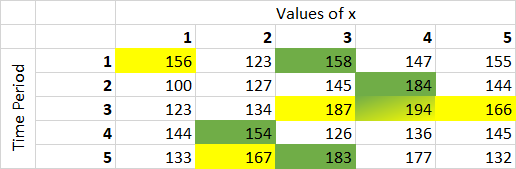
\includegraphics[width=6cm, height=3cm]{pic15}
%    \end{center}
    \item \underline{Assumptions}: in order to solve the Bellman Equation we need to impose the following assumptions
    \begin{itemize}
        \item  \underline{Assuumption 1}: the Bellman Equation has a unique strictly concave solution
        \item  \underline{Assumption 2}: the solution is approached in the limit as $j \rightarrow \infty$ by iterations on
        \begin{gather*}
            V_{j+1}(x) = \max_{u} \left\{r(x,u) + \beta V_{j}(\widetilde{x}) \right\}
        \end{gather*}
        Subject to $\widetilde{x} = g(x,u)$, $x$ given, and starting from any bounded and continuous initial $V_{0}$. Note that $\widetilde{x}$ is tomorrows $x$
        \item  \underline{Assumption 3}: there is a unique and time-invariant optimal policy of the form $u_{t} = h(x_{t})$, where $h$ is chosen to maximize the RHS of the Bellman equation
        \item  \underline{Assumption 4}: off the corners, the limiting value function $V$ is differentiable
    \end{itemize}
    \item  \underline{Solution}: the Bellman Equation and the Policy Function are the building blocks for constructing the optimal solution
    \begin{itemize}
        \item  \underline{Step 1 - Backward Induction}: compute $\{ V_{t} (x) \}_{t=0}^{T}$ and $\{ U_{t} (x) \}_{t=0}^{T−1}$ by backward induction using the Bellman Equation
        \begin{itemize}
            \item \underline{Part 1}: compute $V_{t}(x) = W(x) \ \forall x \in \mathfrak{X}$
            \item  \underline{Part 2}: for all $t = T − 1, T −2, \dots, 0$ compute $V_{t}(x) = \max_{u} \{ r(x,u) + \beta V_{t+1} (g(x, u)) \}$ and $U_{t}(x) = \arg \max_{u} \{ r(x,u) + \beta V_{t+1} (g(x, u)) \}$ for all $x \in \mathcal{X}$
            \item \underline{Example}
            \begin{gather*}
                \boxed{t=T} \\
                \forall x^{i}, \ \begingroup\color{magenta} V_{T}(x^{i}) \endgroup = W(x^{i}) \rightarrow \ \text{final condition} \\
                \\
                \boxed{t=T-1} \\
                \forall x^{i}, \ V_{T-1}(x^{i}) = \max_{u} \left\{ r(x^{i}, u) + \beta \begingroup\color{magenta} V_{T}(x^{i}) \endgroup \right\} \\
                U_{T-1}(x^{i}) = \arg \max_{u} \left\{ r(x^{i}, u) + \beta V_{T}(x^{i}) \right\} \\
                \dots \\
                \text{repeat these steps until we reach} \ \boxed{t=0}
            \end{gather*}
            Note that because the state variable x is discrete, we know how many times we need to iterate backwards until $t=0$
        \end{itemize}
        \item  \underline{Step 2 - Iterating Forward}: given $x_{0}$ compute $\{u_{t}^{*}\}_{t=1}^{T−1}$ and $\{x_{t}^{*}\}_{t=1}^{T}$ by iterating forward on $$\{ U_{t} (x) \}_{t=0}^{T−1}$$
        \begin{itemize}
            \item \underline{Method}: we iterate forward using $x$
            \begin{gather*}
                u_{0}^{*} = U_{0}(x_{0}^{*}), \ \ \tikzmark{a}x_{1}^{*} = g(x_{0}^{*}, u_{0}^{*}), \\
                u_{1}^{*} = U_{1}(x\tikzmark{b}_{1}^{*}), \ \ x_{2}^{*} = g(x_{1}^{*}, u_{1}^{*}), \\
                \dots \\
                u_{t}^{*} = U_{t}(x_{t}^{*}), \ \ x_{t+1}^{*} = g(x_{t}^{*}, u_{t}^{*}), \\
                \dots \\
                u_{T-1}^{*} = U_{T-1}(x_{T-1}^{*}), \ \ x_{T}^{*} = g(x_{T-1}^{*}, u_{T-1}^{*}),
                \begin{tikzpicture}[overlay,remember picture,-latex,shorten >=0.001pt,shorten <=0.001pt]
                    \draw[->,red, distance=0.25cm] (a.south) to (b.north west);
                \end{tikzpicture}
            \end{gather*}
            \item \underline{Intuition}: the law of motion will indicate what the future value of $x_{t}$ is given the control variable $u$, allowing us to derive the solution. Note that the control variable $u$ is able to be calculated due to having previously found the value of $u$ via backward induction in step 1
        \end{itemize}
    \end{itemize}
\end{itemize}
\vspace{2.5mm}
\par \underline{Infinite Horizon Problem}: consider the problem \begin{gather*}
\max_{\{u_{t}\}_{t=0}^{\infty}} \ \sum_{t=0}^{\infty} \beta^{t}r(x_{t}, u_{t}) \\
\text{subject to}: \ x_{t+1} = g(x_{t}, u_{t}), \ \ \ x_{0} \text{is given}
\end{gather*}
We want to compute the solution $\{u_{t}^{*}, x_{t+1}^{*}\}_{t=0}^{\infty}$
\begin{itemize}
    \item \underline{Assumptions}: in addition to the previous finite horizon problem assumptions we assume that $r(\cdot)$ is bounded, also note that now the bellman equation is a functional equation in V
    \item  \underline{No Backward Induction}: since there is no terminal condition to start with (ie V is time-invariant) we cannot use backward induction
    \item \underline{Conditions for a Solution}: the following four conditions must hold for the infinite horizon problem to be solved
    \begin{itemize}
        \item \underline{Condition 1}: the Bellman Equation has a unique strictly concave solution $V^{*}$
        \item \underline{Condition 2}: let $V^{0}$ be any bounded and continuous VF and let $V^{j}$ satisfy
        \begin{gather*}
            V^{j}(x) = \max_{u} \left\{ r(x,u) + \beta V^{j-1}(g(x,u)) \right\} \ \ \text{for} \ j \geq 1
        \end{gather*}
        Then $V^{*} = \lim_{j \rightarrow \infty} V^{j}$
        \item \underline{Condition 3}:There is a unique and time-invariant policy function $U^{*}$ such that the solution to the original problem can be obtained by iterating on $u^{*}_{t} = U^{*}(x_{t})$
        \item \underline{Condition 4}: off the corners, the limiting value function $V^{*}$ is differentiable with
        \begin{gather*}
            V^{*'}(x) = r_{1}(x, U(x)) + \beta V^{*'}(g(x,U(x)))g_{1}(x,U(x))
        \end{gather*}
    \end{itemize}
    Note that the second condition implies that if you have any function $V_{0}$ that is bounded and continuous then if you iterate on $j$ you will eventually find the solution $V^{*}$ (ie a steady state). The third condition implies that from finding $V^{*}$ you can use $u_{*}$ to then backwards iterate to find $U^{*}$
    \item  \underline{Guess and Verify Method}: also known as the method of undetermined coefficients, this involves guessing and verifying a solution $V$ to the Bellman Equation. This relies on the uniqueness of the solution to the Bellman Equation (condition 1) and can be solved analytically with pen and paper (though does not always work)
        \begin{itemize}
            \item  \underline{Step 1}: guess that the true value function has a particular parametric form $V^{G}(x; A)$ where A is a vector of unknown parameters
            \item  \underline{Step 2}: compute $\widehat{V}(x;A) = \max_{u} \{r(x,u) + \beta V^{G}(g(x,u);A) \}$
            \begin{itemize}
                \item \underline{Note}: you can solve for the control variable that is implied by the policy function by using the FOC (provided in condition 4). This then allows you to solve for the optimized $\widehat{V}(x;A)$
            \end{itemize}
            \item  \underline{Step 3}: if there exists parameters $A^{*}$ such that $\widehat{V}(x; A^{*}) = V^{G}(x;A^{*})$ then $V^{G}(x;A^{*})$ is the solution
            \begin{itemize}
                \item \underline{Note}: compare the derived optimized value function $\widehat{V}(x;A)$ from step 2 to $V^{G}(x; A)$
            \end{itemize}
        \end{itemize}
    \item \underline{Value Function Iteration Method}: we proceed by constructing a sequence of value functions and associated policy functions. The sequence is created by iterating on the following equation, starting from $V_{0} = 0$, and continuing until $V_{j}$ has converged:
    \begin{gather*}
        V_{j+1}(x) = \max_{u} \left\{r(x,u) + \beta V_{j} (\widetilde{x}) \right\} \\
        \text{subject to} \ \ \ \widetilde{x} = g(x,u), \ x \ \ \text{given}
    \end{gather*}
     This method always works because by solution method condition 2 we have $V^{*} = \lim_{j \rightarrow \infty} V^{j}$, however this method can be very slow particularly for problems with more than one state
    \begin{itemize}
        \item  \underline{Step 1}: start from any bounded and continuous guess $V^{0}$
        \item  \underline{Step 2}: iterate on $V^{j}(x) = \max_{u} \{ r(x,u) + \beta V^{j−1} (g(x,u)) \}$ until convergence (ie until $||V^{j} − V^{j−1}|| < \varepsilon$)
    \end{itemize}
    \item  \underline{Policy Function Iteration Method}
    \begin{itemize}
        \item  \underline{Step 1}: pick a feasible policy function $U^{0}(x)$ (or $u = h_{0}(x)$) and compute the value associated with operating forever with that policy
        \begin{gather*}
            V_{h_{j}}(x) = \sum_{t=0}^{\infty} \beta^{t} r [x_{t}, h_{j}(x_{t})]
        \end{gather*}
        where $x_{t+1} = g[x_{t}, h_{j}(x_{t})]$ with $j=0$
        \item  \underline{Step 2}: generate a new policy $u = h_{j+1}(x)$ that solves the two period problem
        \begin{gather*}
            \max_{u} \left\{r(x,u) + \beta V_{h_{j}} [g(x,u)]\right\}
        \end{gather*}
        for each x
        \item  \underline{Step 3}: iterate over j until convergence, repeating steps 1 and 2
    \end{itemize}
    \item  \underline{Example}: consider a social planner solving
    \begin{gather*}
    \max_{\{c_{t}, k_{t+1} \}_{t=0}^{\infty}} \ \sum_{t=0}^{\infty} \beta^{t} \ln (c_{t}) \\
    \text{subject to}: \ c_{t} + k_{t+1} = Ak_{t}^{\alpha}, \ \ \ k_{0} \ \text{is given}
    \end{gather*}
    where $\alpha \in (0,1)$ and $\beta \in (0,1)$
    \begin{itemize}
        \item \underline{Simplification}: rearranging the constraint and substituting $$c_{t}$$ into the objective function we have
        \begin{gather*}
        \max_{\{k_{t+1} \}_{t=0}^{\infty}} \ \sum_{t=0}^{\infty} \beta^{t} \ln (Ak_{t}^{\alpha} − k_{t+1}) \\
        \text{subject to}: \ k_{0} \ \text{is given}
        \end{gather*}
        Here the State Variable is $t \rightarrow k^{t}$ (i.e. today's capital) and the control variable is $t \rightarrow k_{t+1}$ (i.e. tomorrow's capital). Note that indexes have been dropped since it is an infinite horizon problem with k being the state and k' being the control. The Bellman Equation given this simplication is
        \begin{gather*}
            V(k) = \max_{k^{'}} \{ \ln(Ak^{\alpha} − k^{'}) + \beta V(k^{'}) \}
        \end{gather*}
        \item  \underline{Guess and Verify Solution}: here we guess the functional form $V^{G}(k; E, F) = E + F \ln (k)$ where E and F are unknown constants. We then plug in $V^{G}(x; E, F)$ into the RHS of the Bellman equation yielding
        \begin{gather*}
            \widehat{V}(k; E, F) = \max_{k} \Big\{ \ln(Ak^{\alpha} - k^{'}) + \beta V^{G}(k^{'}; E, F) \Big\} = \max_{k} \Big\{ \ln(Ak^{\alpha} - k^{'}) + \beta(E + F \ln (k)) \Big\}
        \end{gather*}
         Taking first order conditions and log-linearizing results in the optimal policy function $k^{'}(k) = \frac{\beta F}{1 + \beta F}Ak^{\alpha}$. Substituting the optimal policy function into the objective function yields
         \begin{gather*}
             \widehat{V}(k;E,F) = \underbrace{\bigg[ \ln \Big(\frac{A}{1+\beta F} \Big) + \beta F \ln \Big( \frac{\beta F}{1 + \beta F} A \Big) + \beta E \bigg]}_{E^{'}} + \underbrace{\alpha(1+\beta F) \ln(k)}_{F^{'}} \\
             \Updownarrow \\
             \widehat{V}(k; E^{'}, F^{'}) = E^{'} + F^{'} \ln(k)
         \end{gather*}
         When grouping the constants for $\widehat{V}(k; E’, F’)$ it has the same functional form as $V^{G}(k; E, F)$. Finally, we pin down the unknown coefficients by solving the system of equations
         \begin{align*}
             E^{*} &= \bigg[ \ln \Big(\frac{A}{1+\beta F} \Big) + \beta F \ln \Big( \frac{\beta F}{1 + \beta F} A \Big) + \beta E \bigg] \\
             F^{*} &= \alpha(1+\beta F) \ln(k)
         \end{align*}
         Note that the equation for $E^{*}$ is derived from collecting constant terms and $F^{*}$ is derived from collecting the terms containing our dependent variable. This leaves us with the final solution $V^{*} = E^{*} + F^{*} \ln (k)$ and the optimal policy function $k^{'*}(k) = \frac{\beta F^{*}}{1 + \beta F^{*}} A k^{\alpha}$
         \begin{itemize}
             \item \underline{Solution Write Out}: here the Bellman Equation is $V(k) = \max_{k^{'}} \left\{ \ln(A k^{\alpha} - k^{'}) + \beta V(k^{'}) \right\}$
             \begin{itemize}
                 \item  \underline{Step 1}: my guess is $V^{G} (k) = F \ln (k) + E$ where $F$ and $E$ are our unknown constants
                 \item  \underline{Step 2}: using my guess we have
                 \begin{gather*}
                     \widehat{V}(k) = \max_{k^{'}} \Big\{ \ln(Ak^{\alpha} - k’) + \beta (Ak^{\alpha} - k’) \Big\} = \max_{k^{'}} \Big\{ \ln(Ak^{\alpha} - k^{'}) + \beta(E + F \ln (k^{'})) \Big\}
                 \end{gather*}
                 Taking first order conditions we have the following
                 \begin{gather*}
                    -\frac{1}{Ak^{\alpha}-k^{'}} + \beta F \frac{1}{k^{'}} = 0 \\
                    \Downarrow \\
                    k^{'} = \frac{\beta F}{1 + \beta F} Ak^{\alpha} \tag{$\star$}
                 \end{gather*}
                 Plugging $\star$ into the objective function, we obtain the optimized value function $\widehat{V}(k)$
                 \begin{gather*}
                     \widehat{V}(k;E,F) = \underbrace{\bigg[ \ln \Big(\frac{A}{1+\beta F} \Big) + \beta F \ln \Big( \frac{\beta F}{1 + \beta F} A \Big) + \beta E \bigg]}_{E^{'}} + \underbrace{\alpha(1+\beta F)}_{F^{'}} \ln(k)
                 \end{gather*}
                 \item  \underline{Step 3}: to evaluate the parameters $(E^{*}, F^{*})$ we solve the system of equations implied by the functional form
                 \begin{align*}
                     \widehat{V}(k) &= E^{'} + F^{'} \ln (k) \\
                     V^{G}(k) &= E + F \ln(k)
                 \end{align*}
             This yields
                 \begin{align*}
                     E^{'} = E &\Rightarrow E = \ln \Big(\frac{A}{1+\beta F} \Big) + \beta F \ln \Big( \frac{\beta F}{1 + \beta F} A \Big) + \beta E \\
                     F^{'} = F &\Rightarrow F = \alpha(1+\beta F)
                 \end{align*}
                 Note that by $F = \alpha(1+\beta F)$ and $F^{'} = F$ we have $F^{*} = \tfrac{\alpha}{1 - \alpha \beta}$ which gives us the policy function with one unknown $k^{'*}(k) = \tfrac{\beta F^{*}}{1 + \beta F^{*}} A k^{\alpha}$
             \end{itemize}
         \end{itemize}
    \end{itemize}
\end{itemize}
\vspace{2.5mm}
\par \underline{Stochastic Problems}: consider the stochastic problem
\begin{gather*}
\max_{\{ u_{t} \} ^{\infty}_{t=0}} \mathbb{E}_{0} \sum_{t=0}^{\infty} \\
\text{subject to}: \ x_{t+1} = g(x_{t}. U_{t}, \varepsilon_{t+1}), \ \ \ \text{given} \ x_{t}
\end{gather*}
\begin{itemize}
    \item  \underline{iid Shocks}: $\varepsilon_{t}$ is a sequence of iid shocks with the cumulative distribution function $\Pr [\varepsilon_{t} \leq e ] = F(e)$
    \begin{itemize}
        \item \underline{Timing}: $\varepsilon_{t+1}$ is realized at $t+1$ after $u_{t}$ has been chosen, therefore $x_{t}$ is a sufficient statistic at $$t$$
        \item \underline{iid Assumption}: this is important for recursive formulation for if shocks were persistent instead then the state vector should also incorporate past shock realizations
    \end{itemize}
    \item \underline{Bellman Equation}: the Bellman Equation for this problem is
    \begin{gather*}
        V(x) = \max_{u} \{ r(x,u) + \beta \mathbb{E}[V(g(x,u, \varepsilon))|x] \}
    \end{gather*}
    where $\mathbb{E} [V(g(x, u, \varepsilon))|x ] = \int V(g(x,u,\varepsilon))dF(\varepsilon)$ and $V(x)$ is the optimal value of the problem starting from $x$ at $t=0$
    \item \underline{Solution Methods}: the previous solution methods still apply and the solution $V(x)$ of the Bellman Equation can be computed by iterating on
    \begin{gather*}
        V_{j+1}(x) = \max_{u} \left\{r(x,u) + \beta \mathbb{E} \bigg[ V_{j}[g(x,u,\varepsilon) | x] \bigg] \right\}
    \end{gather*}
    starting from any bounded continuous initial $V_{0}$.
    The first order necessary condition for the problem on the RHS of the Bellman Equation is
    \begin{gather*}
        r_{2}(x,u) + \beta \mathbb{E} \left\{V^{'} [g (x, u, \varepsilon)] g_{2}(x,u,\varepsilon) | x \right\} = 0
    \end{gather*}
    which we obtain simply by differentiating the Bellman Equation and passing the differentiation operation under the $\mathbb{E}$ (an integration) operator. Off corners, the value function satisfies
    \begin{gather*}
        V^{'}(x) = r_{1}[x, h(x)] + r_{2}[x, h(x)]h^{'}(x) + \beta \mathbb{E}\left\{ V^{'} \{g [x, h(x), \varepsilon] \} \{g_{1}[x,h(x), \varepsilon] + g_{2}[x, h(x), \varepsilon]h^{'}(x) \} | x \right\}
    \end{gather*}
    When the states and controls can be defined in such a way that $x$ does not appear in the transition equation, the formula for $V^{'}$ becomes
    \begin{gather*}
        V^{'}(x) = r_{1}[x, h(x)]
    \end{gather*}
    Substituting this formula into the first order necessary condition for the problem gives the stochastic Euler equation
    \begin{gather*}
        r_{2}(x,u) + \beta \mathbb{E} [r_{1}(\widetilde{x}, \widetilde{u})g_{2}(x, u, \varepsilon) | x] = 0
    \end{gather*}
    where tildes over $x$ and $u$ denote next period values.
    \begin{itemize}
        \item \underline{Integral Valuation}: the integral in expectation can be approximated by quadrature, if closed form solutions are infeasible
    \end{itemize}
\end{itemize}

\newpage

\section{Dynamic Optimisation in Continuous Time}

\par \underline{\bf{Continuous vs Discrete Time}}: in discrete time the intervals between periods are $\Delta>0$ (e.g. the interval between $t$ and $t+1$ is 1), in continuous time the intervals between periods are $\Delta \rightarrow 0$
\begin{itemize}
    \item  \underline{Continuous Variables Issue}: while state variables are often naturally continuous, when using computational methods we can only evaluation the value function  on a finite number of points. Since continuous variables are not countable this becomes an issue
    \begin{itemize}
        \item \underline{Solution}: we can address this problem via using (1) discretization of the state space, or, (2) polynomial approximation to the value function
    \end{itemize}
\end{itemize}
\vspace{2.5mm}
\par \underline{\bf{Discretization Method}}: consider a problem with continuous state and control variables $\mathfrak{x} \in \mathbb{R}$, discretization just replaces $\mathfrak{x}$ and $\mathfrak{u}$ by the finite grids $\widehat{\mathfrak{x}} = \{ x^{1}, \dots, x^{n} \}$ and $\widehat{\mathfrak{u}} = \{ u^{1}, \dots, u^{n} \}$. Here we discretize for a vector of unknown capital levels $k = [0, k_{1}, \dots, \overline{k}]$, we need to decide how big of a grid should we create when discretizing
\begin{itemize}
    \item \underline{Value Function Impact}: now the value function becomes a finite list of numbers, $V = [V^{1}, \dots, V^{n}]^{T}$
    \item  \underline{Advantage}: the maximization step is much simpler than under the original bellman equation, which is a key advantage of discretization methods
    \item  \underline{Disadvantage}: there is a "curse of dimensionality" in muiltidimensional state spaces where we can have either $N$ points for a one-dimensional state space vs $N^{k}$ points for a k-dimensional state space, which increases the number of states.
    \begin{itemize}
        \item  \underline{Grid Decision}: requires some a-priori information about the state space, which is sometimes difficult to obtain (e.g. upper and lower bounds). Typically, you choose a steady state level of capital and then select the grid up to that steady state
    \end{itemize}
    \item  \underline{Optimal Growth Illustration}: suppose $V(k) = \max_{k'} \left\{ \ln (Ak^{\alpha} - k') + \beta V(k') \right\}$ where in this case $\mathfrak{x} = \mathfrak{u}$
    \begin{itemize}
        \item \underline{Discretization}: if we discretize $\mathfrak{x}$ then the Bellman equation becomes $V_{i} = \max_{j} \left\{ \ln (Ak^{\alpha}_{i} - k_{j}) + \beta V_{j} \right\}$ for all $i = 1, \dots, n$ where $i$ indexes the different possible current levels of capital and $j$ indexes the different possible levels of future capital
        \item \underline{Value Function Iteration Illustration}: suppose we applied value function iteration and therefore iterate on the mapping $V_{i}^{s} = \max \left\{ \ln(Ak^{\alpha}_{i} - k_{1}) + \beta V_{1}^{s-1}, \dots, \ln(Ak_{i}^{\alpha} - k_{n}) + \beta V_{n}^{s-1} \right\}$ for all $i = 1, \dots, n$ where $s$ indexes the iteration step
        \begin{itemize}
            \item \underline{Step 1}: start with a guess
            \begin{gather*}
                v_{n \times 1}^{0} = \begin{bmatrix} v_{1}^{0} \\ v_{2}^{0} \\ \dots \\ v_{n}^{0} \end{bmatrix}, \ \ \ \text{where} \ \ v_{i}^{0} \equiv v^{0}(k_{i})
            \end{gather*}
            Note that our guess on $V^{0}$ has a dimension of $N \times 1$ which is the vector of all values of $v_{0}$ given different levels of capital. Therefore you have $N \times 1$ guesses
            \item \underline{Step 2}: find $V^{1}$ by solving $V_{i}^{1}=\max_{j} \left\{ \ln(Ak_{i}^{\alpha} - k_{j}) + \beta V_{j}^{0} \right\}$ where
            \begin{gather*}
                V_{i}^{1} = \max \begin{bmatrix} \ln(Ak_{i}^{\alpha} - k_{i}) + \beta V_{1}^{0} \\ \ln(Ak_{i}^{\alpha} - k_{2}) + \beta V_{2}^{0} \\ \dots \\ \ln(Ak_{i}^{\alpha} - k_{n}) + \beta V_{n}^{0} \end{bmatrix} \ \ \ \forall i, \ \ \ \text{which reduces to} \ \ \ V_{n \times 1}^{1} = \begin{bmatrix} V_{1}^{1} \\ V_{2}^{1} \\ \dots \\ V_{n}^{1} \end{bmatrix}
            \end{gather*}
            \begin{itemize}
                \item \underline{Note}: $V_{j}^{1}$ is the maximum element contained in the  $N \times 1$ vector of $v_{n \times 1}^{1}$'s. Note that this involves just picking the maximum possible element in the $v_{i}^{1}$ vector containing every possible level of capital for today (ie period $i$)
            \end{itemize}
            \item \underline{Step 3}: check for convergence, setting the tolerance level to the euclidean norm
            \begin{itemize}
                \item \underline{Tolerance Level($\varepsilon$)}: $||v^{1} - v^{0}||< \varepsilon$ where $\varepsilon = \sqrt{\sum_{i=1}^{n}(v_{i}^{1}-v_{i}^{0})}$
            \end{itemize}
            \item  \underline{Step 4}: compute $v^{s}$ by solving $v_{i}^{s} = \max \left\{ \ln(Ak_{i}^{\alpha} - k_{j}) + \beta v_{j}^{s-1} \right\} \ \ \ \forall i$
            \item  \underline{Step 5}: check convergence $||v^{s} - v^{s-1}||< \varepsilon$, if convergence holds then stop else go back to step 2 and iterate again
        \end{itemize}
    \end{itemize}
\end{itemize}
\vspace{2.5mm}
\par \underline{\bf{Ordinary Differential Equations (ODEs)}}: a "differential" equation" is one where the unknown is a function (instead of a variable) and the equation includes one or more of the derivatives of the function, an "ordinary differential equation" equation is one for which the unknown is a function of only one variable (typically time). The order of an ODE is that of the highest derivative - i.e. if the highest derivative is an ODE of order n then it is an nth-order ODE. The goal when solving an ODE is to find the behaviour of of the equation with respect to the unknown (i.e. how it evolves with time)
\begin{itemize}
    \item \underline{Partial ODEs}: where the unknown is a function of more than one variable
    \item  \underline{First-Order ODE Form}: $\dot{x}(t) = F(t, x(t))$, where $\dot{x}(t) \equiv dx(t)/dt$ and $t \in [t_{a}, t_{b}]$
    \begin{itemize}
        \item \underline{Unknown}: here the unknown is a function $x(t)$ with $x: [t_{a}, t_{b}] \rightarrow \mathbb{R}$ and can be found (without uniqueness) by integrating and combining with a initial condition
        \item  \underline{Uniqueness}: the solution is not unique with the form having infinitely many solutions indexed by an integrating constant C. However, generally the constant C can be uniquely determined by requiring the solution to pass through a given point on the $x(t)$-plane, providing us with a general and particular solution
        \item  \underline{Example}: $\dot{x}(t) = 2t$ with $t \in [0,\infty)$ where the dot on top of $x(t)$ represents the derivative of $x(t)$ with respect to time
        \begin{itemize}
            \item \underline{Solution without Initial Condition}: the general solution is $x(t) = t^{2} + C$
            \item  \underline{Solution with Initial Condition}: suppose we impose the initial condition $x(0) = 1$, therefore $C=1$ and the particular solution is $x(t) t^{2} + 1$
            \newline
            \begin{center}
            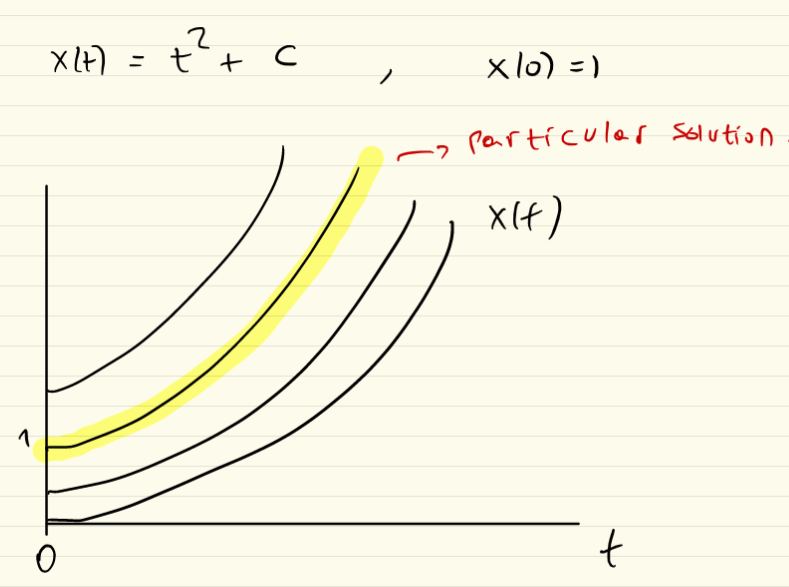
\includegraphics[width=4cm, height=3cm]{pic5}
            \end{center}
        \end{itemize}
    \end{itemize}
    \item  \underline{Finite-Difference Methods for Solution}: here we approximate derivates using finite-differences to approximate the solution to the ODE. This involves finding $\dot{x}(t) = F(t,x(t))$, $x(t_{a}) = x_{a}$, and $t \in [t_{a}, t_{b}]$. There are a wide range of methods depending on how the derivatives are approximated
    \begin{itemize}
        \item  \underline{Euler's Method}: given the equation implied by the ODE
        \begin{itemize}
            \item  \underline{Step 1}: specify a grid for t, i.e. $t_{0} = t_{a} < t_{1} < t_{2} < \dots < t_{N} = t_{b}$
            \item  \underline{Step 2}: we can approximate the ODE using the difference equation $$\frac{x(t_{i+1}) - x(t_{i})}{t_{i+1}-t_{i}} = F(t_{i},x(t_{i}))$$ iterating over $i = 0, \dots, N-1$, where $x(t_{0})=x_{a}$ is fixed by the initial condition
                \begin{itemize}
                    \item  \underline{Note}: the difference equation is obtained by rearranging the equation in step 1, we know all elements on the RHS of the difference equation which provides us with an explicit solution for $x(t_{1})$
                \end{itemize}
        \end{itemize}
        \item  \underline{Euler's Method Illustration}:
        \begin{itemize}
            \item  \underline{Step 1}: discretize $[t_{a}, t_{b}]$
            \item  \underline{Step 2}: iterate forward on $x(t_{i_1}) = x(t_{i}) + (t_{i+1} - t_{1})F(t_{i}, x(t_{i})) \ \ \ \forall i$
            \begin{itemize}
                \item \underline{i=0}: $x(t_{1}) = x(t_{0}) + (t_{1} - t_{0})F(t_{0}, x(t_{0}))$
                \item  \underline{i=1}: $\dots$ (etc)
            \end{itemize}
        \end{itemize}
        \item  \underline{Euler's Method Numerical vs Analytical Solution Equivalency}: $\dot{x}(t) = 2t, \ \ x(0)=1, \ \ t \in [0, 1000]$
            \newline
            \begin{center}
            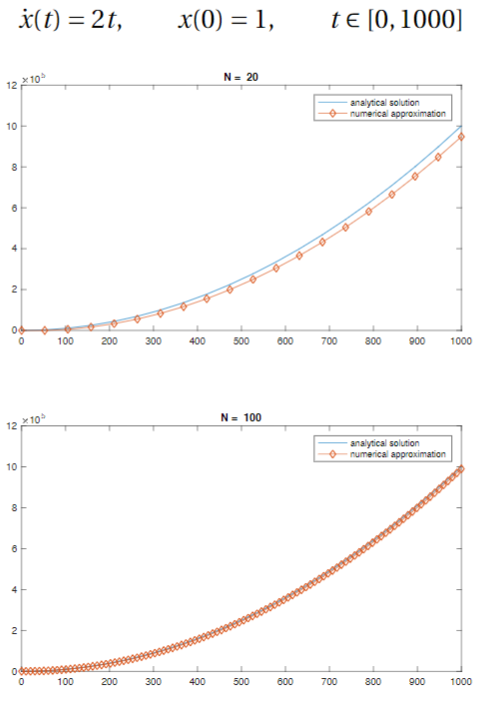
\includegraphics[width=5cm, height=3cm]{pic6}
            \end{center}
    \end{itemize}
    \item \underline{ODE Systems}: consider the system of two equations in two unknowns
    \begin{gather*}\dot{x}(t) = f(t, x(t), y(t)) \\ \dot{y}(t) = g(t, x(t), y(t)) \end{gather*} where $t \in [t_{a}, t_{b}]$. The general solution typically depends on two arbitrary constants,  say A and B, and can be written as \begin{gather*} x(t) = \phi_{1} (t; A, B) \\ y(t) = \phi_{2} (t; A,B) \end{gather*} Here the two arbitrary constants  A and B can be pinned down via two conditions on the solution which causes two types of problems emerge. In other words, the function must be solved such that both the initial and boundary conditions hold. Note that, like single-equation ODEs, exact solutions ODE systems can only be obtained under special cases
    \begin{itemize}
        \item \underline{Initial Value Problem(IVP)}: where you have conditions on the initial time ($a$) values - here $x(t_{a}) = x_{a}$, $y(t_{a}) = y_{a}$ can be solved numerically by applying Euler's Methods
        \begin{itemize}
            \item \underline{Step 1}: discretize the domain
            \item  \underline{Step 2}: iterate forward starting from $x(t_{a}) = x_{a}$ and $y(t_{a}) = y_{a}$
        \end{itemize}
        \item  \underline{Boundary Value Problem (BVP)}: where you have a condition on the value at a time period ($b$) that different from the initial time value ($a$) - here $x(t_{a}) = x_{a}$, $y(t_{b}) = y_{b}$ can be solved by applying a shooting algorithm
        \begin{itemize}
            \item \underline{Step 1}: make an initial guess for $y(t_{a})$ called $y_{a}^{G}$
            \item \underline{Step 2}: solve the ODE system by applying Euler's method given $x(t_{a}) = x_{a}$ and $y(t_{a}) = y_{a}^{G}$
            \item \underline{Step 3}: if $y(t_{b})$ is 'close enough' to $y_{b}$ then stop, else update $y_{a}^{G}$ and go back to step 2
            \newline
            \begin{center}
            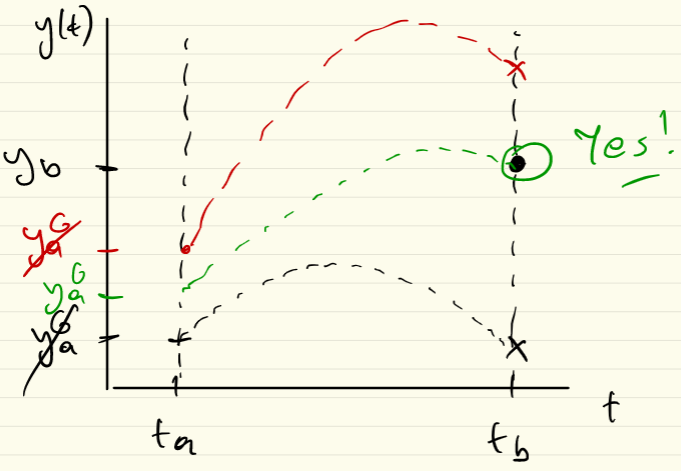
\includegraphics[width=4cm, height=3cm]{pic8}
            \end{center}
            \begin{itemize}
                \item  \underline{Note}: the solution must cause the value of $y(t)$ to equal the a-priori $y(a)$ at time $t_{a}$ and the a-priori $y(b)$ at time $t_{b}$
            \end{itemize}
        \end{itemize}
    \end{itemize}
    \item \underline{Higher-Order ODEs}: techniques for solving ODE systems also apply to analysing higher-order Equations. Here we can express the second order ODE equation as a first order ODE system
    \begin{itemize}
        \item \underline{Example}: consider the second-order ODE \begin{gather*} \ddot{x}(t) = f(t, \dot(t), x(t)) \end{gather*} where $\ddot{x}(t) \equiv \partial^{2}x(t) / \partial t^{2}$.
        Define the new variables $y = \dot{x}$ and you are left with the two-equation ODE system
        \begin{gather*} \dot{y} (t) = f(t, y(t), x(t)) \\ \dot{x}(t) = y(t) \end{gather*}
    \end{itemize}
\end{itemize}
\vspace{2.5mm}
\par \underline{\bf{The Maximum Principle}}: the typical continuous time optimization problem is
\begin{gather*} \max_{x(t), y(t)} \ \int_{0}^{t_{1}} f (t,x(t), y(t)) \ \ \ dt \end{gather*}
subject to
\begin{gather*} \dot{x}(t) = g\big(t, x(t), y(t)\big), \ \ \ x(t) \in \mathcal{X} \ \forall t, \ \ \ y(t) \in \mathcal{Y} \ \forall t, \ \ \ x(0) = x_{0} \end{gather*}
There are two main issues with conventional solution methods to this problem; (1) we are choosing over infinitely dimensional objects such as the function $x: [0, t_{1}] \rightarrow \mathcal{X}$, (2) the constaints include a differential equation rather than a set of equalities/inequalities. In order to overcome these issues and find a solution, we apply the maximum principle theorem
\begin{itemize}
    \item \underline{Notation and Assumptions}: $x$ is the state variable, $y$ is the control variable, $\mathcal{X} \subset \mathbb{R}$  and $\mathcal{Y} \subset \mathbb{R}$ are nonempty and convex, $f$ and $g$ are continuously differentiable in their arguments, we define a Hamiltonian, and for simplicity we assume $t_{1} < \infty$
    \begin{itemize}
        \item  \underline{Hamiltonian}: we define the hamiltonian $$H(t,x(t),y(t),\mu(t)) \equiv f(t,x(t),y(t)) + \mu(t)g(t,x(t),y(t))$$ where $\mu(t)$ is a continuously differentiable function called the costate variable
    \end{itemize}
    \item  \underline{Maximum Principle Theorem}: suppose that the aforementioned continuous time problem has an interior continuous solution $(\widehat{x}(t), \widehat{y}(t))$. Then there exists a continuously differentiable function $\mu(t)$ such that
    \begin{gather*} H_{y}(t,\widehat{x}(t), \widehat{y}(t), \mu(t)) = 0 \ \ \forall t \in [0, t_{1}] \\ \dot{\mu}(t) = -H_{x}(t, \widehat{x}(t), \widehat{y}(t), \mu(t)) \ \ \forall t \in [0, t_{1}] \\ \mu(t_{1}) = 0 \end{gather*}
    \begin{itemize}
        \item \underline{ODE Usage}: by $H_{y}(t,\widehat{x}(t), \widehat{y}(t), \mu(t)) = 0$ we can solve for $y$ as a function of $x$ thereby writting $y = Y(t, x \mu)$. Plugging $y = Y(t, x \mu)$ into $\dot{\mu}(t) = -H_{x}(t, \widehat{x}(t), \widehat{y}(t), \mu(t))$ and $ \dot{x}(t) = g\big(t, x(t), y(t)\big)$ and combining the law of motion we are left with
        \begin{gather*} \dot{x} = g\big(t, x, Y(t,x,\mu)\big) \\ \dot{\mu} = -H_{x}\big(t,x,Y(t,x,\mu),\mu \big) \\ x(0) = x_{0}, \ \ \ \mu(t_{1}) = 0 \end{gather*}
        which is an ODE system in $x$ and $\mu$ that can be solved numerically by applying the shooting algorithm
        \item \underline{Sufficient Condition Requirements}: the maximum principle only provides necessary conditions for an optimum, sufficient conditions for a maximum rely on concavity properties of the objective and on convexity of the feasible set
        \item \underline{Technique Generalization}: the techniques generalize to multidimensional problems (where $x$ and $y$ are vectors), infinite horizon problems (ie $t_{1} = \infty$), and to including terminal conditions on the final state (e.g. $x(t_{1}) = x_{1}$)
        \item \underline{Index}: the variable t may represent time or any other index
    \end{itemize}
\end{itemize}
\vspace{2.5mm}
\par \underline{\bf{Heuristic Proof of The Maximum Principle}}: to solve problem $(x)$ it would be natural to start trying "some sort" of lagrangian optimization such as constructing the function \begin{gather*} \mathcal{L} = \int_{0}^{t_{1}} \left\{F(t, x(t), y(t)) + \mu(t)[g(t,x(t), y(t)) - \dot{x}(t)] \right\} \end{gather*} where $\mu(t)$ is a continuously differentiable function from the hamiltonian. Supposing that $(\widehat{x}(t), \widehat{y}(t))$ is an interior solution to the lagrange problem, then $(\widehat{x}, \widehat{y})$ should maximize $\mathcal{L}$.
\begin{itemize}
    \item \underline{Lemma}: the function $\mathcal{L}$ can be written as \begin{gather*} \mathcal{L} = \int_{0}^{t_{1}} \left\{ f(t,x(t),y(t)) + \mu(t)g(t,x(t),y(t)) + \dot{\mu}(t)x(t) \right\} \ \ dt - \mu(t_{1})x(t_{1}) + \mu(0) x(0) \end{gather*}
    \begin{itemize}
        \item \underline{Proof}: note that
        \begin{gather*} \int_{0}^{t_{1}} \tfrac{\partial (\mu(t)x(t))}{\partial t} \ \ dt = \int_{0}^{t_{1}} \dot{\mu}(t)x(t) \ \ dt + \int_{0}^{t_{1}} \mu(t)\dot{x}(t) \ \ dt
        \end{gather*}
        If we integrate both sides over $[0, t_{1}]$ then we have
        \begin{gather*}
            \mu(t_{1})x(t_{1}) - \mu(0)x(0) = \int_{0}^{t_{1}} \dot{\mu}(t) x(t) \ \ dt + \int_{0}^{t_{1}} \mu(t)\dot{x}(t) \ \ dt
        \end{gather*}
        This can be rearranged as
        \begin{gather*} \mu(t)\dot{x}(t) \ \ dt = \mu(t_{1})x(t_{1}) - \mu(0)x(0) - \int_{0}^{t_{1}} \dot{\mu}(t)x(t) \ \ dt
        \end{gather*}
        Plugging this into our lagrangian yields the above lemma
    \end{itemize}
    \item \underline{Proof of Function Features}: consider a variation/perturbation around the optimal path $(\widehat{x}(t), \widehat{y}(t))$. Specifically, take an arbitrary function $P_{y}(t)$, let $\varepsilon \in \mathbb{R}$, and define $y(t, \varepsilon) = \widehat{y}(t) + \varepsilon P_{y}(t)$. Here$y(t, \varepsilon)$ is the solution plus a deviation from the solution ($\widehat{y}(t) + \varepsilon P_{y}(t)$) Graphically
    \newline
    \begin{center}
    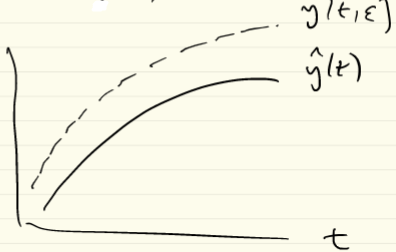
\includegraphics[width=4cm, height=3cm]{pic9}
    \end{center}
    Similarly, let $x(t, \varepsilon) = \widehat{x}(t) + \varepsilon P_{x}(t)$ where $P_{x}(t)$ denotes the corresponding perturbation to $\widehat{x}(t)$ when $\widehat{y}(t)$ is varied according to $P_{y}(t)$. Note that the sum of the perturbations is the variation around the optimum. Define the 'perturbed' lagrangian function as
    \begin{gather*}
    \mathcal{L}(\varepsilon) = \int_{0}^{t_{1}} \left\{ f(t,x(t,\varepsilon),y(t,\varepsilon)) + \mu(t)g(t,x(t,\varepsilon),y(t,\varepsilon)) + \dot{\mu}(t) x(t,\varepsilon) \right\} \ \ dt - \mu(t_{1})x(t_{1}, \varepsilon)+\mu(0)x_{0}
    \end{gather*}
    Recall that $\mathcal{L}$ is maximized at $\widehat{x},\widehat{y}$, where the marginal gain from increasing $\varepsilon$ (ie the perturbation) is 0, and therefore we must have
    \begin{gather*}
    \tfrac{\partial \mathcal{L}(\varepsilon)}{\partial \varepsilon} | (\varepsilon, x, y) = (0, \widehat{x}, \widehat{y}) = 0
    \end{gather*}
    Using the definitions of $x(t,\varepsilon)$, $y(t,\varepsilon)$, and $\mathcal{L}$ the above equation can be expressed as:
    \begin{align*}
     0 = &\int_{0}^{t_{1}} \Big\{ \overbrace{f_{x}(t,\widehat{x}(t),\widehat{y}(t)) + \mu(t)g_{x}(t,\widehat{x}(t),\widehat{y}(t))}^{ \begingroup\color{magenta} H_{x}(t,\widehat{x}(t), \widehat{y}(t), \mu(t)) \endgroup} + \dot{\mu}(t) \Big\} P_{x}(t) \ \ dt \\ &+ \int_{0}^{t_{1}} \underbrace{\Big\{f_{y}(t,\widehat{x}(t), \widehat{y}(t)) + \mu(t)g_{y}(t,\widehat{x}(t), \widehat{y}(t)) \Big\} }_{\begingroup\color{magenta}H_{y}(\cdot)\endgroup} P_{y}(t) \ \ dt - \mu(t_{1})P_{x}(t_{1})
    \end{align*}
    \begin{itemize}
        \item  \underline{Note}: this expression can only hold for all feasible perturbation paths $(P_{x}, P_{y})$ if each integrand vanishes and $\mu(t_{1}) = 0$ such that $P_{y}(t)$ and $P_{x}(t)$ equal 0, which are the conditions of the maximum principle
    \end{itemize}
\end{itemize}

\newpage

\section{Enforcement Frictions I}

\vspace{2.5mm}
\par \underline{Overview}: the analysis of contractual arrangements and enforcement frictions aims to rectify conflicts of interest that arise from violations of two assumptions - (1) both parties were perfectly committed to the rules of the exchange, (2) both parties in the exchange shared the same information. Dropping either of these assumptions creates conflicts of interest
\begin{itemize}
    \item  \underline{Assumption 1 Violation}: here an agent who is not committed to the rules of the exchange would deviate from such rules when she finds it more convenient
    \item  \underline{Assumption 2 Violation}: here an agent who possesses private information would manipulate such information to her advantage
\end{itemize}
\vspace{2.5mm}
\par \underline{Contract Theory}: the study of the economic aspects of contract design where a contract is a set of rules that facilitates cooperation among individuals with conflicting objectives. The goal of contract theory is twofold with the normative goal of how to draw up better contracts and the positive goal of analysing why real life contracts have various forms and designs. We can arbitrarily classify contract theory models by two classifications - (1) according to the type of private information, (2) according to the duration of the contractual relationship
\begin{itemize}
    \item \underline{Type of Private Information}: here we assume that the uninformed party designs the contract and address two types of information issues (adverse selection and moral hazard)
    \begin{itemize}
        \item  \underline{Adverse Selection}: asymmetric information about the characteristics of the informed party (e.g. life insurance where the insured's state of health is unknown by the insurer)
        \item  \underline{Moral Hazard}: asymmetric information about the actions of the informed party (e.g. CEO compensation where the CEO's actions are imperfectly observed by the Board of Directors)
    \end{itemize}
    \item  \underline{Duration of Contractual Relationship}: here we address two types of contract periods (static and dynamic)
    \begin{itemize}
        \item  \underline{Static Contracts}: relationship lasts for one period
        \item  \underline{Dynamic Contracts}: relationship lasts for more than one period (gives rise to enforcement/commitment issues)
    \end{itemize}
\end{itemize}
\vspace{2.5mm}
\par \underline{Principal-Agent Paradigm}: since contracts involve two parties we need to address how the parties bargain over  the terms of the exchange. We bypass the difficulties inherent to the bargaining process by allocating all bargaining power to one of the parties (the Principal) who will offer a take-it or leave-it contract to the Agent. The Principal-Agent Paradigm is the norm in contract theory
\begin{itemize}
    \item \underline{w.l.o.g}: the set of Pareto optimal contracts can be characterised by maximizing the utility of one agent subject to a given level of utility of the other agent. This outcome is a result of the Principal-Agent analogy
\end{itemize}
\vspace{2.5mm}
\par \underline{Enforcement Frictions}: occur when agents are free to walk away from the contract at any time, note that for most models of enforcement frictions we assume that all information is public
\begin{itemize}
    \item  \underline{One-Sided Limited Commitment}: occurs when the principal is committed but the agent is not
    \begin{itemize}
        \item \underline{Applications}: long term labour contracts (principal is the firm and agent is the worker), international lending (principal is the lending country and agent is the borrowing country), firm dynamics (principal is the bank, agent is the entrepreneur seeking to finance a project)
    \end{itemize}
\end{itemize}
\vspace{2.5mm}
\par \underline{One-Sided No Commitment Model}: the economy lasts for $T = \infty$ periods and consists of a village with a large number of households. Household preferences are
\begin{gather*}
    U = \mathbb{E}_{0} \sum_{t = 0}^{\infty} \beta^{t} u(c_{t})
\end{gather*}
where $\beta \in (0, 1)$ and $u$ is concave and has the usual properties. Each HH receives a stochastic endowment stream $\left\{y_{t}\right\}_{t=0}^{\infty}$ where $y_{t} \in \left\{ \overline{y}_{1}, \overline{y}_{2}, \dots, \overline{y}_{S} \right\}, \overline{y}_{s+1} > \overline{y}_{s}$. HHs can only trade with a risk-neutral moneylender who can borrow or lend at the risk free rate $R = \beta^{-1}$. The moneylender maximizes the expected present value of profits from making contracts:
\begin{gather*}
    P = \mathbb{E}_{0} \sum_{t=0}^{\infty} \beta^{t} (y_{t} - c_{t})
\end{gather*}
where $(y_{t} - c_{t})$ is the net transfer from HH at time t
\begin{itemize}
    \item \underline{Assumptions}: $y_{t}$ is iid across time and HHs with $\Pr (y_{t} = \overline{y}_{s}) = \Pi_{S}$, s is the set from which you draw your endowment (it is not time nor is it necessarily growing with time), overline represents the realizations of the endowments,   due to concavity HHs value insurance against endowment realizations, $y_{t}$ is non-storage and therefore self-insruance is precluded, a moneylender (ie the planner) is the only person who has access to a risk-free loan market outside the village, HHs cannot trade with one another, $R$ is exogeneous (ie this is a partial equilibrium model)
    \item  \underline{Contract}: a contract between the moneylender and the HH is a sequence of history dependent functions $\left\{c_{t}\right\}_{t=0}^{\infty}$ with $c_{t} = f_{t} (y^{t})$. The contract specifies that in each period the HH contributes her endowment realization $y_{t}$ in exchange for consumption $c_{t}$
    \begin{itemize}
        \item  \underline{Contractual Friction}: the HH can walk away from the contract. If the HH walks away then the HH consumers their endowment and lives in autarky evermore. The HH cannot return from autarky
        \item  \underline{One-Sided No Commitment}: only the HH can break the contract, the moneylender is fully committed to keeping their promise
        \item  \underline{Information is Symmetric}: the moneylender can observe $y_{t}$
    \end{itemize}
    \item  \underline{Optimal Contract Solution}: the optimal contract can be analysed using recursive tools, this relies on knowing the continuation utility under autarky ($v_{aut}$) where:
    \begin{gather*}
        v_{aut} = \mathbb{E}_{0} \sum_{t=0}^{\infty} \beta^{t} u(y_{t}) = \frac{1}{1-\beta} \sum_{s=1}^{S} \Pi_{s} u(\overline{y}_{s})
    \end{gather*}
    where the continuation utility under autarky is the weighted sum of the possible realizations from the endowment (which due to iid we can remove the dependency of $y$ on time). Note that we can use the geometric series transformation to remove the dependency of $\beta$ on time, giving us a time independent equation
    \begin{itemize}
        \item \underline{Participation Contraint}: since autarky is the outside option of the agents, the optimal contract must satisfy the participation constaints where the value of the contract is worth more than the value of autarky (otherwise the HH will default) :
        \begin{gather*}
            u(\overbrace{f_{t}(y^{t})}^{\begingroup\color{magenta} c_{t} \endgroup}) + \underbrace{\beta \mathbb{E}_{t} \sum_{j=1}^{\infty} \beta^{j-1} u(\overbrace{f_{t+j}(y^{t+j})}^{\begingroup\color{magenta} c_{t+j} \endgroup})}_{\begingroup\color{magenta} w_{t}(y^{t}): \ \text{continuation utility at t} \endgroup} \geq u(y_{t}) + \beta v_{aut}
        \end{gather*}
        for all $t, y^{t}$
        A contract that satisfies the participation contraint is said to be self-enforcing. Participation constraints can be written as
        \begin{gather*}
            u(f_{t}(y^{t})) + \beta \begingroup\color{cyan} w_{t}(y^{t}) \endgroup \geq u(y_{t}) + \beta v_{aut}
        \end{gather*}
        for all $t, y^{t}$ where
        \begin{gather*}
            \begingroup\color{cyan} w_{t}(y^{t}) \endgroup \equiv \mathbb{E}_{t} \sum_{j=1}^{\infty} \beta^{j-1} u(f_{t+j} (y^{t+j}))
        \end{gather*}
        is the continuation utility of the agent at time $t$, given endowment history $y^{t}$
        \item  \underline{Moneylender Problem}: each period the money lender chooses how much to give to the HH and how much that they will promise to transfer in the future (which is encoded in $w$). Therefore, the the money lender solves
        \begin{gather*}
            P(v) = \max_{\left\{ c_{s}, w_{s} \right\} } \sum_{s=1}^{S} \Pi_{s} [\overline{y}_{s} - c_{s} + \beta P(w_{s})]
        \end{gather*}
        subject to
        \begin{align*}
            \sum_{s=1}^{S} \Pi_{s} [u(c_{s}) + \beta w_{s}] \geq v & \rightarrow \ \text{Promise Keeping Constraint} \\
            u(c_{s}) + \beta w_{s} \geq u(\overline{y}_{s}) + \beta v_{aut}, \ \ s = 1, \dots, S & \rightarrow \ \text{Participation Constraint}
        \end{align*}
        Here $w_{s} \in [v_{aut}, \overline{v}]$ where $\overline{v}$ is a large number. $w_{s}$ is the promised future transfers from next period onwards while $w$ is the previous promised transfers from last period. We have one state variable, promised utility $v$. The Promise Keeping Constraint states that the amount the HH gets in expectation must be greater than $v$, in other words the moneylender must be able to fulfil the contract. The Promise Keeping Constraint renders the planning problem time-consistent.
        \begin{itemize}
            \item \underline{Promised Utility $w$}: encodes all history dependence in the contract, allowing one to summarize large dimensional shocks and rewards into a single variable - i.e. continuation utility given the history of endowment shocks
            \item  \underline{Characterisation}: it can be shown that the constraint set is convex and P is stictly concave (as well as differentiable). Given this we have the following lemmas that essentially state that agents have incentives to walk away when income realisations are large enough - wherein the participation constraint will bind for a $\overline{y}_{s}$ that is significantly high
            \begin{itemize}
                \item \underline{Lemma 1}: for each $v$, there exists a threshold $\underline{y}(v)$ such that the PC binds binds if and only if $\overline{y}_{s} \geq \overline{y}(v)$
                \item  \underline{Lemma 2}: the threshold $\overline{y}(v)$ is increasing in v
                \item  \underline{Proof}: we write the lagrangian as
                \begin{gather*}
                    \mathcal{L} = \sum_{s=1}^{S} \Pi_{s} [\overline{y}_{s} - c_{s} + \beta P(w_{s})] \\ + \varepsilon \left\{ \sum_{s=1}^{S} \Pi_{s} [u(c_{s}) + \beta w_{s} - v \right\} \\ +  \sum_{s=1}^{S} \eta_{s} \left\{ u(c_{s}) + \beta w_{s} - u(\overline{y}_{s}) - \beta v_{aut} \right\}
                \end{gather*}
                where $\varepsilon$ and $\eta$ are the lagrangian multipliers on the Promise Keeping Constraint and Participation Contraint respectively. Taking first order conditions and applying the envelope theorem yields the following:
                \begin{align*}
                    \frac{\partial \mathcal{L}}{\partial C_{s}} = 0 &\rightarrow -\Pi_{s} + \varepsilon \Pi_{s} u^{'}(C_{s}) + \eta_{s} u^{'} (C_{s}) = 0 \tag{(1)} \\
                    \frac{\partial \mathcal{L}}{\partial w_{s}} = 0 &\rightarrow \eta_{s} + \varepsilon \Pi_{s} = - \Pi_{s}P^{'}(w_{s}) \tag{(2)} \\
                    \text{Envelope Theorem}: \ \ &\rightarrow P'(v) = - \varepsilon < 0 \tag{(3)}
                \end{align*}
                Rearranging equations $(1)$ and $(2)$ for $\varepsilon \Pi_{s} + \eta_{s}$ and solving them simultaneously yields
                \begin{align*}
                    u^{'}(C_{s}) = - P^{'}(w_{s})^{-1} \tag{(4)}
                \end{align*}
                It is clear to see that the LHS of this equation falls with $C_{s}$ due to concavity of $u(\cdot)$ and the RHS of this equation falls with $w_{s}$ due to concavity of $P(\cdot)$. This implies that $C_{s}$ and $w_{s}$ are positively related.
                \newline
                Combining $(3)$ and $(2)$ yields the law of motion for continuation Utility
                \begin{align*}
                    P^{'}(w_{s}) = P^{'}(v) - \frac{\eta_{s}}{\Pi_{s}} \tag{(5)}
                \end{align*}
                \newline
                \underline{Lemma 1 Proof}
                \newline
                Take as given that $\overline{y}_{s}$ subject to PC is not binding (i.e. $\eta_{s} = 0$), therefore by $(5)$ we have
                \begin{gather*}
                    P^{'}(w_{s}) = P^{'}(v) \Rightarrow w_{s} = v \ \ \text{by concavity}
                \end{gather*}
                Using this fact into $(4)$ we can write $c$ as a function of only $v$ and so have
                \begin{gather*}
                    u^{'}(C_{s}) = -P^{'} (v)^{-1}
                \end{gather*}
                Which can be rewritten as $C_{s} = g_{1}(v), \ \ g_{1}^{'} > 0$. This allows us to rewrite the PC as
                \begin{gather*}
                    u(C_{s}) + \beta w_{s} > u(\overline{y}_{S}) + \beta v_{aut} \\
                    \Big\Downarrow \\
                    u(g_{1}(v)) + \beta v > u(\overline{y}) + \beta v_{aut} \equiv \overline{y}(v) \\
                    \Big\Downarrow \\
                    \underbrace{u^{-1} (u(g_{1}(v)) _ \beta (v-v_{aut}))}_{\begingroup\color{cyan} \equiv \overline{y}(v) \endgroup} > \overline{y_{s}}
                \end{gather*}
                Thus, given the definition of $\overline{y}(v)$, the PC is not binding if and only if $\overline{y}_{s} < \overline{y}(v)$
                \newline
                \underline{Lemma 2 Proof}
                \newline
                Given the definition of $\overline{y}(v)$ from the proof for Lemma 1, this is straightforward
                    \newline
                    \begin{center}
                    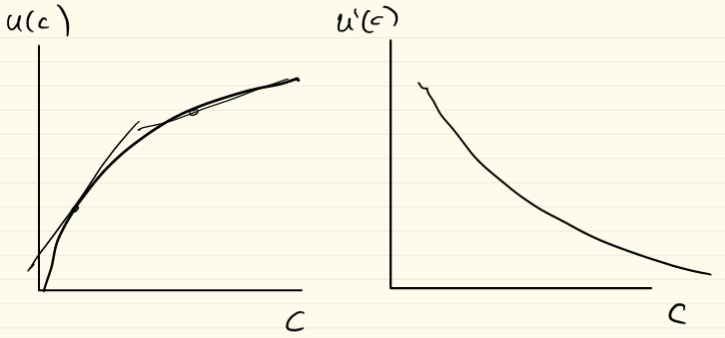
\includegraphics[width=4cm, height=3cm]{pic11}
                    \end{center}
            \end{itemize}
        \end{itemize}
        \item \underline{Properties of PC Binding vs Not Binding}
        Suppose PC is not binding, then $w_{s} = v$ and $C_{s} = g_{1}(v)$ where $g_{1}^{'} > 0$. Therefore, if PC is not binding then $w_{s}$ and $C_{s}$ remain constant
        Suppose PC is binding, then $w_{s} = l(\overline{y}_{s}) > v$ and $C_{s} = g_{2}(\overline{y}_{s}) \in (g_{1}(v), \overline{y}_{s})$ where $l^{'}, g_{2}^{'} \geq 0$. Therefore, if PC is binding then $w_{s}$ and $C_{s}$ must increase to induce the agent not to walk away from the contract - wherein $w_{s}$ and $c_{s}$ only depend on current income realisations (and not on the history of shocks given by  $v$)
        \begin{itemize}
            \item \underline{Consumption under Oprtimal Contract}: graphically, given v, consumption under the optimal contract is
                \newline
                \begin{center}
                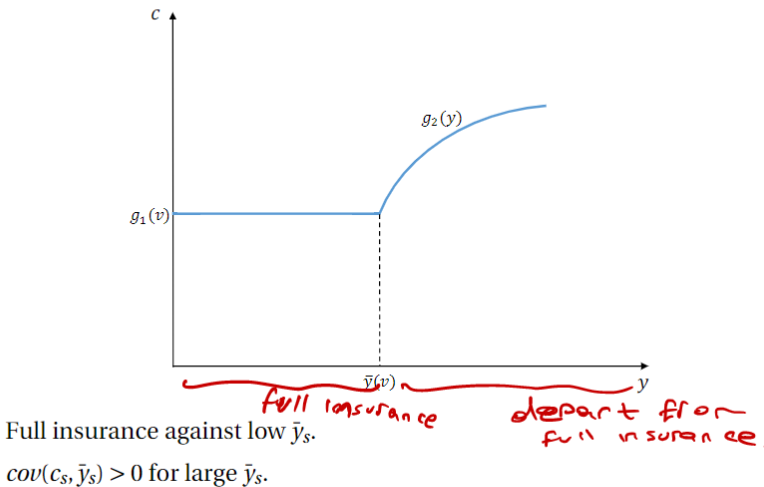
\includegraphics[width=8cm, height=6cm]{pic12}
                \end{center}
            \item \underline{Long Run Dynamics}: $c_{t}$ increases over time until $\overline{y}_{S}$ is realized
                All agents eventually become fully insured (no fluctuations in consumptions) when their highest income realization $\overline{y}_{S}$ is realized and therefore $C$ eventually becomes constant.
                \newline
                \begin{center}
                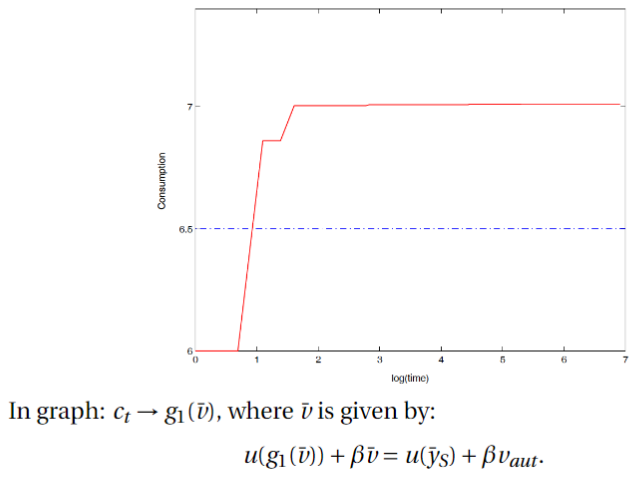
\includegraphics[width=8cm, height=6cm]{pic13}
                \end{center}
                With many HHs, all agents eventually get to consume $g_{1}(\overline{v})$: $\lim_{t \rightarrow \infty} \Pr(c_{t} = g_{1}(\overline{v})) = 1$. Overall, we have "fanning in" of the cross-sectional distribution of consumption and full risk sharing in the long run (ie t=500)
                \newline
                \begin{center}
                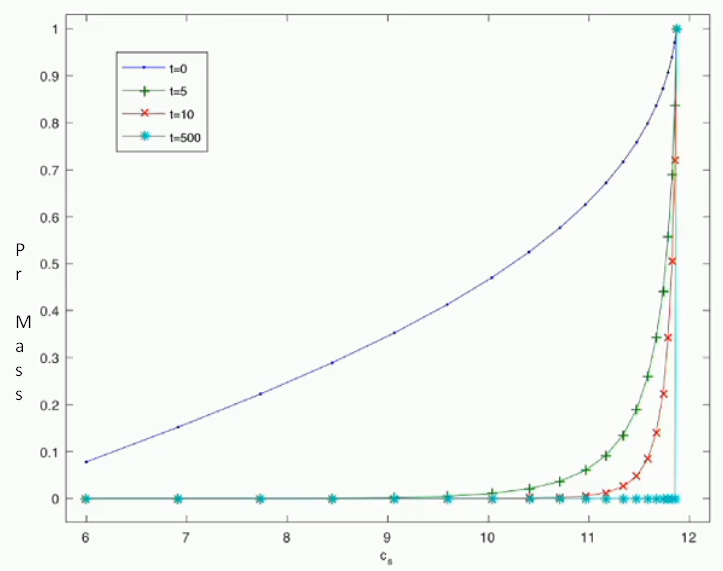
\includegraphics[width=8cm, height=6cm]{pic14}
                \end{center}
            \item  \underline{Not Binding Proof}: shown in the proof of the lemma
            \item  \underline{Binding Proof}: assume that PC is binding
            \begin{itemize}
                \item \underline{Step 1}: show that $w_{s}$ and $c_{s}$ are only functions of $\overline{y}_{s}$
                \newline
                By FOC $(4)$ we have $u^{1} (C_{s}) = -P^{'}(w_{s})^{-1}$ and given the fact that PC is binding we have $u(C_{s}) + \beta w_{s} = u(\overline{y}_{s}) + \beta v_{aut}$. Note that these two equations form a system of 2 equations in 2 unknowns ($C_{s}, w_{s}$). Since promised $v$ does not show up in this system we can write its solution as $w_{s} = \mathcal{l}(\overline{y}_{s})$ and $C_{s} = g_{2}(\overline{y}_{s})$
                \item  \underline{Step 2}: show that $g_{2}^{'} > 0$ and $\mathcal{l}^{'} > 0$
                \newline
                By $u(C_{s}) + \beta w_{s} = u(\overline{y}_{s}) + \beta v_{aut}$ we know that $[u(C_{s}) + \beta w_{s}]$ is non-decreasing in $\overline{y}_{s}$. Also, by $u^{1} (C_{s}) = -P^{'}(w_{s})^{-1}$ (as shown previously), $C_{s}$ is non-decreasing in $w_{s}$ and hence $C_{s}$ should be non-decreasing in $\overline{y}_{s}$
                \item  \underline{Step 3}: show that $w_{s} > v$
                \newline
                By $P^{'}(w_{s}) = P^{'}(v) - \tfrac{\eta_{s}}{\Pi_{s}}$, if the PC binds then $\eta_{s} > 0$ and so $P^{'}(w_{s}) < P^{'}(v) \Rightarrow w_{s} > v$ via concavity
                \item  \underline{Step 4}: show that $C_{s} \in (g_{1}(v), \overline{y}_{s})$
                \newline
                A binding PC implies that $u(C_{s}) + \beta w_{s} = u(\overline{y}_{s}) + \beta v_{aut}$. Therefore, $c_{s} < \overline{y}_{s}$. Because $w_{s} > v$ we have
                \begin{gather*}
                    -P^{'}(w_{s})^{-1} < -P^{'}(v)^{-1} \\
                    \Big\Downarrow \\
                    u^{'}(C_{s}) < u^{'}(g_{1}(v)) \ \ \text{by (4)} \\
                    \Big\Downarrow \\
                    C_{s} > g_{1}(v)
                \end{gather*}
            \end{itemize}
        \end{itemize}
    \end{itemize}
    \item \underline{Connection to Labour Contracts}: early work on one-sided limited commitment models aimed at analysing the characteristics of labour contracts. In our model this can be mapped as $C$ being the wage offered within a firm, $y$ shock being wages offered in the spot market, and the enforcement friction being labour mobility. Since workers are risk-averse, they value insurance against fluctuations in the spot market for wages (i.e. implicit insurance premium in contractual wages). Firms find contractual arrangement beneficial because in the short run they can pay wages below those in the spot market (due to the implicity insurance premium), which is embedded by $C_{s} < \overline{y}_{s}$ when PC binds in our model
\end{itemize}

\newpage


\end{document}
